\documentclass[UTF-8, a4paper, 12pt]{ctexart}

\usepackage[left=1in,right=1in,top=1.00in,bottom=1.00in]{geometry}      % 页边距
\usepackage[colorlinks,linkcolor=blue,anchorcolor=blue,citecolor=green,CJKbookmarks=True]{hyperref}
\usepackage{CJK,CJKnumb}
\usepackage{indentfirst}        % 首行缩进宏包
\usepackage{latexsym,bm}        % 处理数学公式中和黑斜体的宏包
\usepackage{amsmath,amssymb}     % AMSLaTeX宏包 用来排出更加漂亮的公式
\usepackage{graphicx}
\usepackage{cases}
\usepackage{pifont}
\usepackage{txfonts}
\usepackage{subfigure}
\usepackage{pdfpages}
\usepackage{listings}
\usepackage{xcolor}
\usepackage[subfigure]{tocloft}     % 模板中用了subfigure,不加此选项会产生冲突
\usepackage{inconsolata}
\CTEXsetup[format={\Large\bfseries}]{section}%设置章标题字号为Large,居左
\zihao{-4}\linespread{1.5}\selectfont
\renewcommand{\theequation}{\arabic{section}-\arabic{equation}}
\renewcommand{\thefigure}{\arabic{section}-\arabic{figure}}
\renewcommand{\thetable}{\arabic{section}-\arabic{table}}
%\renewcommand{\thefigure}{\thechapter-\arabic{figure}}
\renewcommand{\cftsecleader}{\cftdotfill{\cftdotsep}}
\renewcommand\contentsname{{\qquad\qquad\qquad\qquad\qquad\qquad 目\quad 录}}
\newcommand{\song}{\CJKfamily{song}}    % 宋体   (Windows自带simsun.ttf)
\renewcommand{\abstractname}{\textbf{\large {摘\quad 要}}} %更改摘要二字的样式


%%%%%%%%%%%%%%%%%%%%
% 设置列表行距
\usepackage{enumitem}
\setenumerate[1]{itemsep=0pt,partopsep=0pt,parsep=\parskip,topsep=5pt}
\setitemize[1]{itemsep=0pt,partopsep=0pt,parsep=\parskip,topsep=5pt}
\setdescription{itemsep=0pt,partopsep=0pt,parsep=\parskip,topsep=5pt}
%%%%%%%%%%%%%%%%%%%%%%%
% -- text font --
% compile using Xelatex
%%%%%%%%%%%%%%%%%%%%%%%
% -- 中文字体 --
%\setCJKmainfont{Microsoft YaHei}  % 微软雅黑
%\setCJKmainfont{YouYuan}  % 幼圆
%\setCJKmainfont{NSimSun}  % 新宋体
%\setCJKmainfont{KaiTi}    % 楷体
%\setCJKmainfont{SimSun}   % 宋体
%\setCJKmainfont{FangSong}   % 仿宋
%\setCJKmainfont{SimHei}   % 黑体
 
% -- 英文字体 --
%\setmainfont{Times New Roman}
%\setmainfont{DejaVu Sans}
%\setmainfont{Latin Modern Mono}
%\setmainfont{Consolas}
\setmainfont{CMU Serif}

%%%%%%%%%%%%%%%%%%%%%%%
%  设置水印
%%%%%%%%%%%%%%%%%%%%%%%
%\usepackage{draftwatermark}         % 所有页加水印
%\usepackage[firstpage]{draftwatermark} % 只有第一页加水印
%\SetWatermarkText{Copyright(C) 2021. by HU S K}           % 设置水印内容
% \SetWatermarkText{\includegraphics{fig/ZJDX-WaterMark.eps}}         % 设置水印logo
%\SetWatermarkLightness{00.9}             % 设置水印透明度 0-1
%\SetWatermarkScale{0.4}                   % 设置水印大小 0-1
%%%%%%%%%%%%%%%%%%%%%%%




%%%%%%%%%%%%%%%%%%%%%%%%%%%%%%%%%%%%%%%%%%%
%用来设置附录中代码的样式
% 头文件
%%%%%%%%%%%%%%%%%%%%%%%%%%%%%%%%%%%%%%%%%%%
\usepackage{listings} 
\usepackage{fontspec}
\setmonofont{Consolas}
%\begin{lstlisting}[
%	language = matlab, numbers=left, 
%	numberstyle=\tiny,keywordstyle=\color{blue!70},
%	commentstyle=\color{red!50!green!50!blue!50},frame=shadowbox,
%	rulesepcolor=\color{red!20!green!20!blue!20},
%	basicstyle=\ttfamily,
%	]
%	
%\end{lstlisting}



%\title{\bfseries \Huge  }
%\author{}
%\date{}

\begin{document}
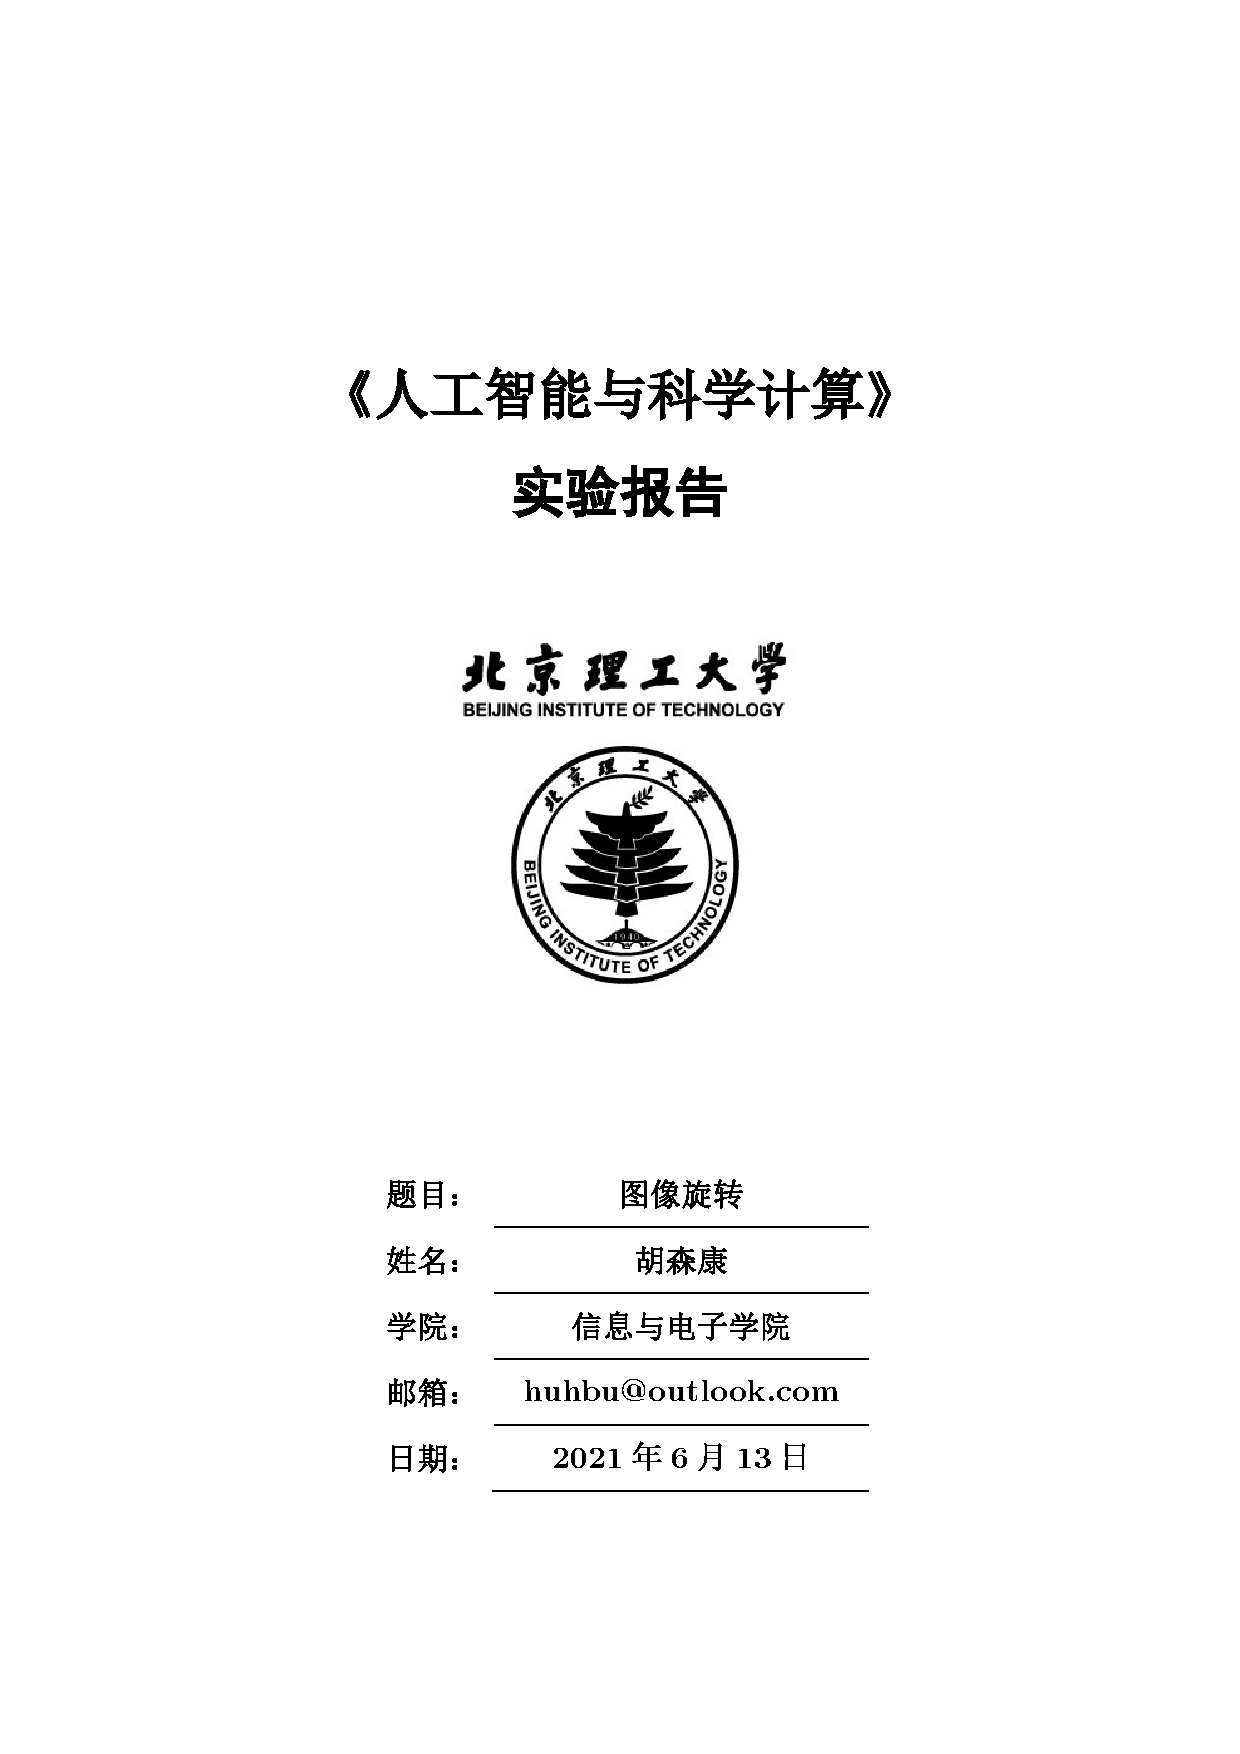
\includepdf[pages={1}]{coverpage.pdf} %% 插入pdf

%\maketitle

%\thispagestyle{empty}
%\newpage
%\thispagestyle{empty}


     

     
%\thispagestyle{empty}       %本页不显示页码
%\newpage                    %分页
\tableofcontents\thispagestyle{empty}
\newpage
\setcounter{page}{1}        %从下面开始编页,页脚格式为导言部分设置的格式

\section{实验目的}
\begin{enumerate}
    \item 采用前向映射和线性插值实现图像旋转,串行
    \item 在1的基础上实现OpenMP并行
    \item 注意各种优化措施
\end{enumerate}

\section{实验原理}

\subsection{图像变换与映射}
我们在进行图像处理时常常需要对图像进行变换。比如对图像进行缩放,旋转,平移等。图像变换的本质是将像素点的坐标通过某一种函数关系,映射到另外的位置。假设变换前图像为$I(x,y)$,变换后图像为$I'(x',y')$,则变换前后的图像之间存在下列关系:
\begin{gather}
    \left[\begin{array}{c}
        x'\\y'
    \end{array}\right]=
    \left[\begin{array}{c}
        f(x,y)\\g(x,y)
    \end{array}\right]\label{e1}\\
     I(x,y)=I'(x',y')=I\left(f(x,y),g(x,y)\right)\label{e2}\\
     \left[\begin{array}{c}
        x\\y
    \end{array}\right]=
    \left[\begin{array}{c}
        f^{-1}(x',y')\\g^{-1}(x',y')
    \end{array}\right]\label{e3}\\
    I'(x',y')=I(x,y)=I\left(f^{-1}(x',y'),g^{-1}(x',y')\right)\label{e4}
\end{gather}

式 (\ref{e1}) 和 式 (\ref{e2}) 已知原图像到目标图像的坐标变换($f(x,y),g(x,y)$),因此可以知道原图像的一点在变换后在目标图像的位置,称为前向映射。

相反,式(\ref{e3}) 和 (\ref{e4}) 中已知目标图像的一点 $(x',y')$ 在变换前在原图像上的位置 $(f^{-1}(x′,y′),g^{-1}(x′,y′))$,称为后向映射。

一般认为图像应该绕着中心点旋转,而且图像原点在左上角,计算时首先需要将左上角的远点移动至图像中心,并且将$y$轴翻转。设图像宽为$W$,高为$H$,有
\begin{equation}
    \left[x_1\ y_1\ 1\right]=\left[x_0\ y_0\  1\right]\left[\begin{array}{ccc}
        1&0&0\\
        0&-1&0\\
        -0.5W&0.5H&1
    \end{array}\right]
\end{equation}
由坐标映射关系知,点$(x_1,y_1)$顺时针旋转$\theta$后的坐标$(x_2,y_2)$为:
\begin{equation}
    \left[x_2\ y_2\ 1\right]=\left[x_1\ y_1\ 1\right]\left[\begin{array}{ccc}
        \cos\theta &-\sin\theta&0\\
        \sin\theta&\cos\theta&0\\
        0&0&1
    \end{array}\right]
\end{equation}
若旋转后的图像宽为$W'$,高为$H'$,那么从笛卡尔坐标原点变换回左上角的公式为
\begin{equation}
    \left[x_3\ y_3\ 1\right]=\left[x_2\ y_2\ 1\right]\left[\begin{array}{ccc}
        1&0&0\\
        0&-1&0\\
        0.5W'&0.5H'&1
    \end{array}\right]
\end{equation}
则点$(x_0,y_0)$与顺时针旋转$\theta$角度后的坐标$(x_3,y_3)$之间的关系为:
\begin{equation}\label{forward}
    \left[x_3\ y_3\ 1\right]=\left[x_0\ y_0\  1\right]
    \left[\begin{array}{ccc}
        1&0&0\\
        0&-1&0\\
        -0.5W&0.5H&1
    \end{array}\right]\left[\begin{array}{ccc}
        \cos\theta &-\sin\theta&0\\
        \sin\theta&\cos\theta&0\\
        0&0&1
    \end{array}\right]\left[\begin{array}{ccc}
        1&0&0\\
        0&-1&0\\
        0.5W'&0.5H'&1
    \end{array}\right]
\end{equation}
\begin{equation}\label{backward}
    \left[x_0\ y_0\  1\right]=\left[x_3\ y_3\ 1\right]
    \left[\begin{array}{ccc}
        1&0&0\\
        0&-1&0\\
        -0.5'W&0.5H'&1
    \end{array}\right]\left[\begin{array}{ccc}
        \cos\theta &\sin\theta&0\\
        -\sin\theta&\cos\theta&0\\
        0&0&1
    \end{array}\right]\left[\begin{array}{ccc}
        1&0&0\\
        0&-1&0\\
        0.5W&0.5H&1
    \end{array}\right]
\end{equation}
其中式(\ref{forward})为前向映射公式,式(\ref{backward})为后向映射公式。

\subsection{前向映射}
通常情况下,一个整数位置$(x,y)$经过图像变换后,往往处于非整数的位置,此时要采用插值技术。

如图(\ref{f1})所示,输入图像上整数点坐标映射到输出图像之后,变成了非整数点坐标。因此,需要将像素按照一定的权重分配至其周围四个像素点上。对于输出图像而言,其整数点像素值周围会有很多输入图像像素的映射,每个到其周围的非整数点像素值都会分配一定的灰度值到此整数像素点,将这些分配而来的像素值叠加,就是输出图像整数点位置的像素值。由于这个分配、叠加的特性,前向映射法有时也叫做{\bfseries 像素移交映射}。

\begin{figure}[htbp]
    \centering
    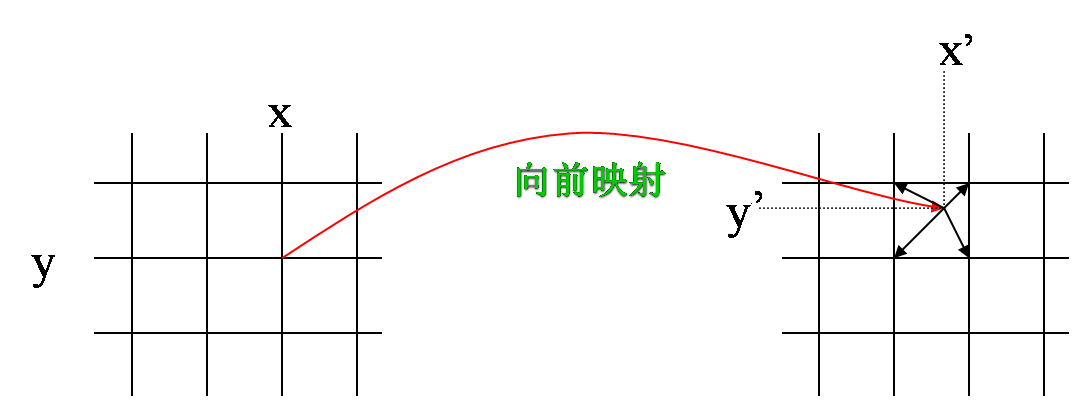
\includegraphics[width=13cm]{fig/f1.jpg}
    \caption{前向映射示意图}
    \label{f1}
\end{figure}

因此,对于前向映射而言,输出图像某一点的像素值不能直接得到,需要遍历输入图像的所有像素值,对其进行坐标变换,分配像素值到整数位置,才能得到输出图像各像素点的像素值,这是前向映射的缺点。

\subsection{后向映射}

相比前向映射,后向映射较为直观。在这种情况下,我们知道输出图像上整数点位置$(x',y')$在变换前位于输入图像上的位置$(x,y)$,一般而言这个是非整数点的位置,利用其周围整数点位置的输入图像像素值进行插值,就得到了该点的像素值。遍历输出图像,经过坐标变换、插值两步操作,就能将其像素值逐个地计算出来,因此向后映射又叫{\bfseries 图像填充映射},如下图(\ref{f2})所示。
\begin{figure}[htbp]
    \centering
    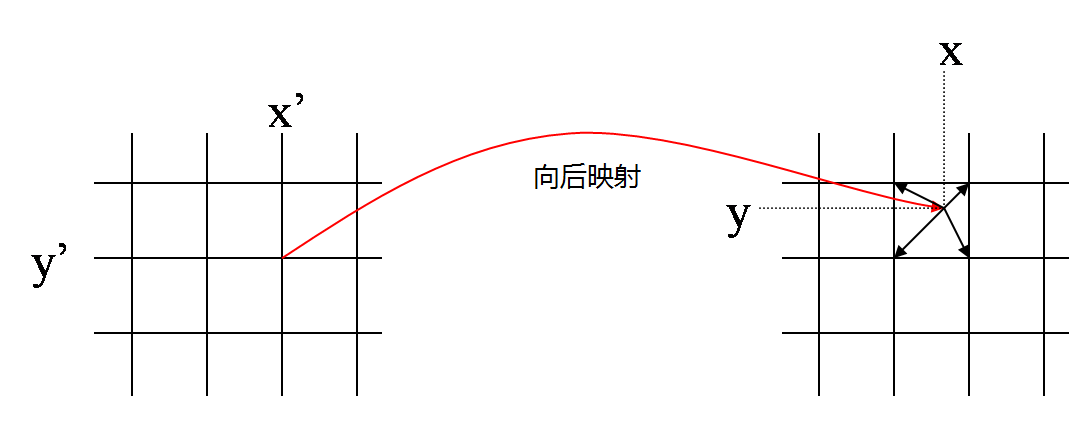
\includegraphics[width=13cm]{fig/f2.jpg}
    \caption{后向映射示意图}
    \label{f2}
\end{figure}

\subsection{插值算法}

常使用的插值算法为{\bfseries 双线性插值},其示意图如下图(\ref{f3})所示。
\begin{figure}[htbp]
    \centering
    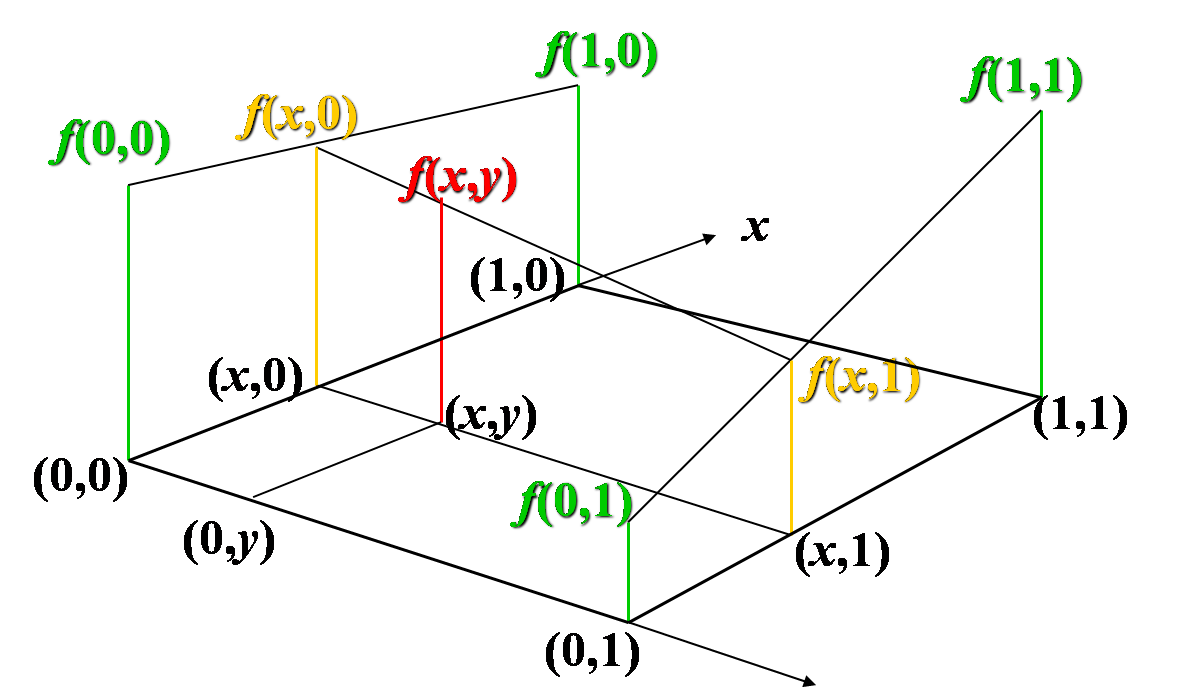
\includegraphics[width=10cm]{fig/f3.jpg}
    \caption{双线性插值算法示意图}
    \label{f3}
\end{figure}

对于后向插值而言,这种情况下输出图像上某点的像素值$I'(x',y')$映射到$f(x,y)$,而$f(x,y)$由输入图像上四点像素值叠加而成。
\begin{equation}
    f(x,y)=(1-x)(1-y)f(0,0)+(1-x)yf(0,1)+x(1-y)f(1,0)+xyf(1,1)
\end{equation}

很容易验证四个权重系数之和为1,插值后图像亮度不变。

对向前插值,输入图像某点$I(x,y)$变换到输出图像$(x',y')$的位置,因此需要将其像素值分配到$f(0,0)$,$f(0,1)$,$f(1,0)$,$f(1,1)$四个位置。分配方式为:
\begin{align}
    f(0,0)&=(1-x)(1-y)f(x,y)\\
    f(0,1)&=(1-x)yf(x,y))\\
    f(1,0)&=x(1-y)f(x,y)\\
    f(1,1)&=xyf(xy)
\end{align}

对于前向映射而言,虽然分配系数和为1,但输出图像上每个点的像素值是多个分配值叠加而成的,因此不能保证多有分配到其上的权重之和为1。因此必须记录下所有分配到其上的权重并累加起来,最后利用累加权重进行\textbf{归一化},才可以得到正确的插值结果。


\subsection{OpenMP基本概念}
OpenMP是一种用于共享内存并行系统的多线程程序设计方案,支持的编程语言包括C、C++和Fortran。OpenMP提供了对并行算法的高层抽象描述,适合在多核CPU机器上的并行程序设计。编译器根据程序中添加的pragma指令,自动将程序并行处理,使用OpenMP降低了并行编程的难度和复杂度。当编译器不支持OpenMP时,程序会退化成普通(串行)程序。程序中已有的OpenMP指令不会影响程序的正常编译运行。


OpenMP采用fork-join的执行模式。开始的时候只存在一个主线程,当需要进行并行计算的时候,派生出若干个分支线程来执行并行任务。当并行代码执行完成之后,分支线程会合,并把控制流程交给单独的主线程。
一个典型的fork-join执行模型的示意图如下图(\ref{f4})所示:
\begin{figure}[htbp]
    \centering
    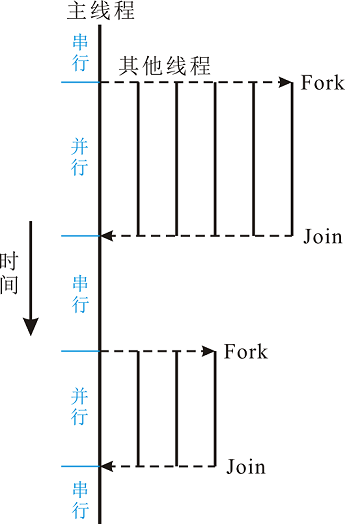
\includegraphics[width=5cm]{fig/f4.png}
    \caption{典型的fork-join执行模型的示意图}
    \label{f4}
\end{figure}

OpenMP编程模型以线程为基础,通过编译制导指令制导并行化,有三种编程要素可以实现并行化控制,他们分别是编译制导、API函数集和环境变量。

\subsection{OpenMP编译指导}
编译制导指令以 \#pragma omp 开始,后边跟具体的功能指令,格式如:\#pragma omp 指令[子句[,子句] …]。
\begin{enumerate}
    \item 常用的功能指令如下:
\begin{itemize}
    \item parallel:用在一个结构块之前,表示这段代码将被多个线程并行执行;
    \item for:用于for循环语句之前,表示将循环计算任务分配到多个线程中并行执行,以实现任务分担,必须由编程人员自己保证每次循环之间无数据相关性;
    \item parallel for:parallel和for指令的结合,也是用在for循环语句之前,表示for循环体的代码将被多个线程并行执行,它同时具有并行域的产生和任务分担两个功能;
    \item sections:用在可被并行执行的代码段之前,用于实现多个结构块语句的任务分担,可并行执行的代码段各自用section指令标出(注意区分sections和section);
    \item parallel sections:parallel和sections两个语句的结合,类似于parallel for;
    \item single:用在并行域内,表示一段只被单个线程执行的代码;
    \item critical:用在一段代码临界区之前,保证每次只有一个OpenMP线程进入;
    \item flush:保证各个OpenMP线程的数据影像的一致性;
   \item  barrier:用于并行域内代码的线程同步,线程执行到barrier时要停下等待,直到所有线程都执行到barrier时才继续往下执行;
    \item atomic:用于指定一个数据操作需要原子性地完成;
    \item master:用于指定一段代码由主线程执行;
    \item threadprivate:用于指定一个或多个变量是线程专用,后面会解释线程专有和私有的区别。
\end{itemize}

\item 相应的OpenMP子句为: 
\begin{itemize}
    \item private:指定一个或多个变量在每个线程中都有它自己的私有副本;
    \item firstprivate:指定一个或多个变量在每个线程都有它自己的私有副本,并且私有变量要在进入并行域或任务分担域时,继承主线程中的同名变量的值作为初值;
    \item lastprivate:是用来指定将线程中的一个或多个私有变量的值在并行处理结束后复制到主线程中的同名变量中,负责拷贝的线程是for或sections任务分担中的最后一个线程; 
    \item reduction:用来指定一个或多个变量是私有的,并且在并行处理结束后这些变量要执行指定的归约运算,并将结果返回给主线程同名变量;
    \item nowait:指出并发线程可以忽略其他制导指令暗含的路障同步;
    \item num\_threads:指定并行域内的线程的数目; 
    \item schedule:指定for任务分担中的任务分配调度类型;
    \item shared:指定一个或多个变量为多个线程间的共享变量;
    \item ordered:用来指定for任务分担域内指定代码段需要按照串行循环次序执行;
    \item copyprivate:配合single指令,将指定线程的专有变量广播到并行域内其他线程的同名变量中;
    \item copyin:用来指定一个threadprivate类型的变量需要用主线程同名变量进行初始化;
    \item default:用来指定并行域内的变量的使用方式,缺省是shared。
\end{itemize}
\item API函数。除上述编译制导指令之外,OpenMP还提供了一组API函数用于控制并发线程的某些行为,下面是一些常用的OpenMP API函数以及说明:
\begin{itemize}
    \item omp\_in\_parallel:判断当前是否在并行域中
    \item omp\_get\_thread\_num:返回线程号
    \item omp\_set\_num\_threads:设置后续并行域中的线程格式
    \item omp\_get\_num\_threads:返回当前并行区域中的线程数
    \item omp\_get\_max\_threads:获取并行域可用的最天线程数目
    \item omp\_get\_num\_procs:返回系统中处理器的个数
    \item omp\_get\_dynamic:判断是否支持动态改变线程数目
    \item omp\_set\_dynamic:启用或关闭线程数目的动态改变
    \item omp\_get\_nested:判断系统是否支持并行嵌套
    \item omp\_set\_nested:启用或关闭并行嵌套
    
\end{itemize}
\item 环境变量。OpenMP中定义一些环境变量,可以通过这些环境变量控制OpenMP程序的行为,常用的环境变量:
\begin{itemize}
    \item OMP\_SCHEDULE:用于for循环并行化后的调度,它的值就是循环调度的类型;  
    \item OMP\_NUM\_THREADS:用于设置并行域中的线程数;  
    \item OMP\_DYNAMIC:通过设定变量值,来确定是否允许动态设定并行域内的线程数;  
    \item OMP\_NESTED:指出是否可以并行嵌套。
\end{itemize}
\end{enumerate}

\newpage
\section{实验过程}

\subsection{图像旋转}

在进行实验过程中,我们首先设计前向映射的图像旋转程序,在此程序中,不进行线性插值,将映射完的浮点数类型的坐标数值直接变为整数数值。

利用此算法进行实验,将图(\ref{tank})顺时针旋转30度,得到结果如图(\ref{tank_f})所示。可以看到基于此算法旋转过后的图像有明显的锯齿。
\begin{figure}[htbp]
    \centering
    \includegraphics[width=10cm]{fig/tank.bmp}
    \caption{原始图像}
    \label{tank}
\end{figure}
\begin{figure}[htbp]
    \centering
    \includegraphics[height=6cm]{fig/tank_forward.bmp}
    \includegraphics[height=6cm]{fig/tank_forward2.bmp}
    \caption{基于原始旋转算法旋转后图像}
    \label{tank_f}
\end{figure}



\subsection{双线性插值}

为了减少锯齿,提高图像旋转质量,编写线性插值函数,将图片(\ref{tank})顺时针旋转30度,得到结果如图(\ref{t1})所示。
\begin{figure}[htbp]
    \centering
    \includegraphics[height=6cm]{fig/t1.bmp}
    \includegraphics[height=6cm]{fig/t12.bmp}
    \caption{基于前向映射的插值旋转图像}
    \label{t1}
\end{figure}
可以看到图像锯齿明显减少,说明此算法是有效的。


\subsection{OpenMP并行实现图像旋转}

在上述实验的基础上对程序加入OpenMP并行算法,以提高程序运行的效率。根据2.6节中的知识,在程序前加入以下语句来实现OpenMP并行。
\begin{lstlisting}[
	language = c++, numbers=left, 
	numberstyle=\tiny,keywordstyle=\color{blue!70},
	commentstyle=\color{red!50!green!50!blue!50},frame=shadowbox,
	rulesepcolor=\color{red!20!green!20!blue!20},
	basicstyle=\ttfamily,
	]
#pragma omp for schedule(static)
\end{lstlisting}

首先关闭OpenMP并行,运行算法,将$600\times 385$大小的图(\ref{tank})顺时针旋转30度,运行10次,记录每次运行的时间,如下表所示。
\begin{table}[htbp]
    \centering
    \caption{无OpenMP并行时算法的运行时间}
    \begin{tabular}{c|cccccccccc}
        \hline
        次数&1&2&3&4&5&6&7&8&9&10\\
        时间(ms)&4.96&4.96&4.96&4.96&4.96&4.97&4.66&4.41&4.35&4.96\\
        \hline
    \end{tabular}
\end{table}


可见其平均时间为4.82ms。

再开启OpenMP并行,将$600\times 385$大小的图(\ref{tank})顺时针旋转30度,运行10次,记录平均运行时间,并改变并行数,得到平均运行时间如下表(\ref{tq})所示。
\begin{table}[htbp]
    \centering
    \caption{OpenMP并行时算法的运行时间}
    \label{tq}
    \begin{tabular}{c|cccccccccc}
        \hline
        线程数&1&2&3&4&5&6&7&8&9&10\\
        平均时间(ms)&3.39&2.94&2.54&2.46&2.37&2.42&2.26&2.25&2.94&3.09\\
        \hline
        线程数&11&12&13&14&15&16&&&&\\
        平均时间(ms)&3.05&2.91&2.99&2.99&2.82&2.97&&&&\\
        \hline
    \end{tabular}
\end{table}

从数据中可以看出,存在OpenMP并行时比串行时的速度快了40\%,说明并行的资源利用率比串行高很多。同时我们可以看到对于OpenMP并行,其运行速度先增加后减小,说明在并行数较小时,并行对算法处理速度有提高的作用,但在之后由于线程数的增加,线程同步需要的计算量增大,因此导致了速度的下降。同时我们还发现在线程数为12至16时,运行速度基本不变,没有因为增加了线程数就对运行速度有明显的影响,从而达到一个上限。
\section{实验感想}

在本次实验中,首先进行了相关知识的调研,了解了图像前向映射和后向映射的基本原理,并阅读了相关算法,此算法较为简单,但在离工程实际还有一些差距,因为在利用前向映射对图片进行旋转后,其坐标不是整数,如果直接粗暴取整,会导致图片的信息出现丢失,同时导致图片的分辨率下降,这是我们不希望看到的现象。

因此在图像旋转后我们对于其非整数的坐标不能粗暴取整,而是要进行一定的处理,保证图像的信息最大限度的保留,而最常用的方法就是双线性插值法(Bilinear Interpolation),利用双线性插值法成功解决了上述问题,达到了图像旋转后信息的最大保留。最终利用了OpenMP并行技术来进行图像旋转实验,实验结果表示,并行技术确实极大的提高了图像的处理速度。


\end{document}
